%!TEX root = ../../report.tex
\section{Content-based Recommender Systems}
\label{sec:content}

\subsection{The functionality of a content-based RS}
The overall reason to implement a Content-based recommender system is basically the same as for other recommender systems; to deliver a list of recommendations that statistically will be seen as valuable to the user. Where it differentiates itself from others is in the way these recommendations are generated.\newline 

A content-based recommender system will try to recommend items to the user similar to items that the user has either bought or somehow interacted with in the past. In other words, the way the content-based recommender system approaches the recommendation process is by analyzing a set of keywords from previous items preferred by the user, and from this information extract the user's preferences and interests.\newline 
These specific preferences will then be compared with items contained in the system. The result returned from the system is a mathematical indication of the relevance these items will represent to the user. As an example, this could help filter search result for webpages. If a resulting webpage has a negative score in comparison to the users interests, it will simply not be added to the list of recommendations.

\subsection{The architecture and modules of the system}
In this section we will describe the different components which represents the content-based recommender system. In the previous section we explained that it produces the recommendations by creating the user profile containing the user's preferences, then comparing these preferences with the items contained in the system, and finally choosing and presenting the recommended items to the user. \newline
There are three main steps used in this recommendation process, which are described as follows; content analysis, profile learning, and filtering. Figure \ref{contentdescription} illustrates the process and can be used as a reference to better comprehend some of the steps which are further explained below.

\begin{figure}[H]
\centering
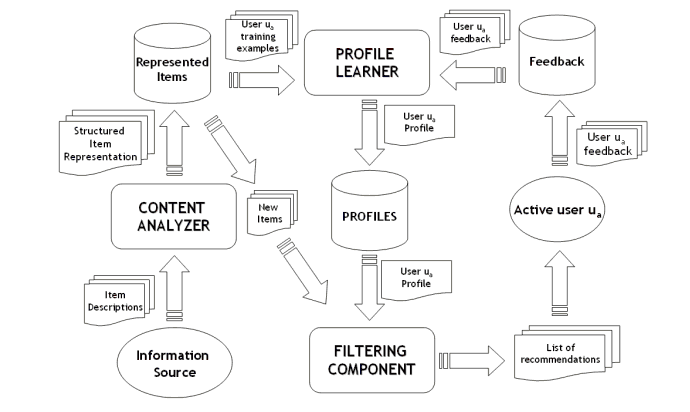
\includegraphics[width=90mm]{Pictures/contentdescription.png}
\caption{source: http://pyevolve.sourceforge.net/wordpress/?p=2497}
\label{contentdescription}
\end{figure}

\begin{itemize}
	\item \textbf{Content Analyzer:} When data has no apparent structure to it, such as text, a processing step which can extract the relevance from the material in a structured way is needed. \newline
	The main responsibility of the Content Analyzer is to represent data (items, webpages, articles, documents, etc.) in such a way, that it can be used by the next processing steps. This is done by shifting the content representation from its original form to a form usable by the target module (this could for instance be a webpage represented as keyword vectors) via a specific extraction technique.
	
	\item \textbf{Profile Learner:} This module collects and utilizes the relevant information that has been analyzed and altered into a usable format by the Content Analyzer. In this case, relevant information is data which represents the users preferences. The profile learner aspires to put this information into the right order, and then use this ordered data to create the user profile for the individual user.
	
	\item \textbf{Filtering Component:} This module uses the profile representation in question and matches this onto the items in the system. These items can, depending on the given context and number of items, be saved in a repository or just held in system memory. The Filtering Component will then sort the items in relation to the user's interests and preferences.\newline
	The result generated gives a statistical indication of how much the user will like the individual items. If there is currently not enough information on the user to give an indication of certain items, then these items can potentially be put on a waiting list until more information on the user is obtained.
\end{itemize}

These three components work together to recommend items to the user via a series of steps. Again refer to figure \ref{contentdescription} for an illustrative overview.\newline 
The first step of the process occurs when the Content Analyzer receives a series of item descriptions from an information source. These descriptions are analyzed in order to extract specific keywords from the unstructured text, to end up with a structured representation of the items. These item representations can then be stored in a repository, which will most often be the case, since this saves time when these items are used again. In order to create and update a user profile for which recommendations are required, the system can collect information on the user's behavior in relation to items and the system in general, giving the system continuous feedback on the user's preferences. This information can also be stored in a repository for future analysis.\newline
During the Profile Learner step, the above mentioned information is processed together with the represented items in order to predict the relevance of these in relation to the user. A user can likewise create a profile where his or her area of interest are directly provided, thus making the feedback part of optional relevance.\newline
There are basically two types of relevant feedback, namely positive and negative. The positive feedback indicates features that the user are interested in, whereas the negative feedback is an indicator of features that have no interest to the user. \newline
These types of feedback can be recorded with two different feedback techniques, namely implicit and explicit feedback. Explicit feedback refer to when the user actively makes a decision, such as a rating or evaluation, about a specific item. Implicit feedback refers to when the user does not make any active involvement, and is captured by monitoring and analyzing the user's activities and behavior.\newline
The explicit feedback technique is the easiest way for the recommender system to make recommendations, since it gives a clear and actual indication of the users preferences. When speaking about the explicit kind of feedback, there are three main approaches: like/dislike, ratings, and comments on items.\newline
The first option works as a binary scale where the user can either choose to like or dislike an item.The rating option gives the user a larger scale to rate an item on, for instance from 1-10, where 10 could indicate the most-liked option. The last option presents the user with a set of text comments from other users in order to aid the user in the decision-making whether to buy or not buy a specific item.\newline

All of the above mentioned actions will help the Profile Learner to create a more comprehensive overview of the users preferences. An advantage of the explicit feedback is that it simplifies the interpretation process of the recommender system for the items in question. A disadvantage can be that the user is required to make an active choice, hence incurring a cognitive load on the user. The implicit feedback is centered around actions that do not require direct user involvement on a cognitive level, but more on their actions in relation to the items in question, such as saving, discarding, bookmarking, etc.\newline

In order for the recommender system to create a user profile, it is needed by the system to first create something called a training set consisting of the current items in the system. This training set is then used by the Profile Learner to match up against the user's preferences in order to build a solid foundation for the user profile. The training set of recommendations is updated on a regular basis in order to keep the recommendations as close to the users current preferences as possible. This is of particular importance since a users preferences are most likely to be in a dynamic state of change over time. Future items which is added to the system will be matched against the user item preferences via the Filtering Component and, if there is a match, these items will be added to the training set and shown as recommendations to the user. \\
In the next section we will discuss how the similarity of items in relation to user preferences are calculated.

\subsection{Keyword-based Vector Space Model}
The mathematical way in which most content-based recommender systems defines the relevance of an item is by the Vector Space Model(VSM), which is a spatial representation of text documents. In this model, each of the documents is represented by a vector in a \(n\)-dimensional space where \(n\) represents the number of keywords from that particular document that matches a, for the system, overall vocabulary.\newline
When using VSM to represent the weight of keywords in documents, there are two things that are important: giving a weight of the keyword which indicates the importance of the keyword in relation to the document it is in and measure the importance of the document in relation to all the other documents contained in the system. A weighting scheme which can be used for this is TD-IDF weighting. \newline

\textbf{TD-IDF} stands for Term Frequency / Inverse Document Frequency. TF-IDF as a whole is used to generate a weight for a specific keyword in a specific document. TF-IDF is divided into two parts.\newline 
The first part is Term Frequency which counts the number of occurrences of a specific keyword in the document being analyzed, and gives this keyword a weight of importance in relation to the keyword in the document with the maximum number of occurrences. TF can also be divided by document length, in order to make sure that a book which have the keyword in it eight times, is not favored over a short document which contains the same keyword four times, since a short document with four occurrences might be of a bigger value to the user than an entire book with only eight occurrences. 
The second part is Inverse Document Frequency which analyzes how many documents contains this term. The formulas for these calculations will be explained further below in this section. \newline
If a keyword happens to be experienced or noted quite often over a series of analyzations of several objects, then this specific keyword will not be given too much weight, since the system see it as common. On the other hand, if a keyword is distinguishable by it occurring infrequently in the documents as a whole, but frequently in specific documents it will achieve a higher weight and can hence be beneficial in order to recommend more precise items in relation to the users preferences.\newline

The document profile is generated by checking the object keywords, which can originate from metadata or the document itself. These keywords are then given a weight in relation to their significance.
The user profile is generated by the system by checking the keywords for the objects that the user has previously interacted with (bought, viewed, tagged, etc.). Each of the object and user profiles are represented by a vector, which consists of the weight of the keywords contained in the profiles. The concept of vector weighting and how the vectors are computed will be further described below.
The vectors of the object profile and the user profile (the user profile can contain vectors for several different areas) are compared by the system by calculating the angle between them. The smaller the angle, the more aligned the item are with the user interests. In many recommender systems, instead of the angle, the Cosine to the angle is used, which gives a value from 0 to 1. This means, that the closer the value is to 1, the more the vectors are aligned.\newline

In order to understand the concept of the vector weighting we imagine that we have a content space that holds all the keywords that are relevant to the specific situation that we are in. In this space, each keyword represents its own dimension (there are as many dimensions as there are keywords in the object). Each of the objects and the user profiles in the system are represented by a vector in this content space.

There are several ways in which a vector can be computed. Here we will outline the three most common ways.
In some cases a vector will represent a fact (true/false statement) and can be computed simply by using a boolean value. An example of this can be whether a specific keyword is used in a specific document, or whether a specific actor is in a specific movie. The boolean would be used here because it is simply not possible to give this vector a further notion of intensity.\newline
Another way to compute a vector can be by the number of keyword occurrences, which can help give a bigger notion of intensity for the vector.\newline
A third way is to use the TF-IDF which implements both of the above mentioned methods, since it gives us a notion of intensity along with a notion of distinctiveness for the individual vector.\newline

Below is shown the formulas for TF-IDF along with an explanation of each.

TF calculates a value for a specific keyword in relation to how many times it occur in the specific document and how many times the most frequently used keyword occur.
%TF
\[
	\text{TF}(t_{k},d_{j}) = \frac{f_{k,j}}{max_{z}f_{z,j}}
\]

The TF-IDF approach adds an extra layer to the TF, by further calculating the keywords occurrences in relation to all documents in the system.
%TF-IDF
\[
	\text{TF-IDF}(t_{k},d_{j}) = \text{TF}(t_{k},d_{j}) * log{\frac{N}{n_{k}}}
\]

Cosine normalization is used to give all the weights in the calculation a value between 0 and 1, and will ensure that the documents are represented by vectors bounded to the same similarity function(between 0 and 1).
%cosine normalization
\[
	w_{k,j} = \frac{\text{TF-IDF}(t_{k},d_{j})}{\sqrt{\sum_{s=1}^{|T|} \text{TF-IDF}(t_{s}, d_{j})^2}}
\]

The cosine similarity is used to indicate the similarity between two vectors, which then can be used to predict whether a user will be interested in a particular item or not. The result is a value between 0 and 1, where 1 indicating a big similarity between the items.

%cosine similarity
\[
	sim({d_{i},d_{j}}) = \frac{\sum_{k}w_{ki}*w_{kj}^2}{\sqrt{\sum_{k}w_{ki}^2}*\sqrt{\sum_{k}w_{kj}^2}}
\]


While some of the challenges of recommender systems is to figure out the right weights and factors to use to compute the recommendations for the users, most of the basic recommender system does not handle interdependencies, since it most often are outside the scope of the systems work area.\newline
An example of an interdependency could be from the movie world where a user might like comedies with violence, and historical documentaries, but do not like historical comedies or violent documentaries (or likes Sean Connery in action movies and Owen Wilson in comedies, but not vice versa). \newline
Since we can state that the vectors in this case would be comedies, violence, historical, and documentaries, the system in its simplicity will have no chance of interpreting the relationship of the users actual preferences, since the system does not have the notion of multiplying different dimensions together. If taking interdependencies into account is a necessity, it is possible to implement this by using a method called LSI/SVD, which stands for Latent Semantic Indexing/Singular Value Decomposition. LSI/SVD identifies associations and patterns between terms and keywords in a text, and adds an extra dimension to the precision with which it is possible to recommend objects to users. LSI/SVD lies beyond the scope of this report and we will not go any further into the functionality of it.\newline

The methods described in this section is essential for a content-based recommender system since they are the foundation on which the recommendations are made.

\subsection{Advantages and disadvantages}
When looking at recommender systems from a content-based systems point of view there are several advantages over a recommender system in a collaborative-based form.\newline

The three main areas of advantage are user independence, transparency, and new items.\newline
The user independence shows itself in that the content-based recommendations are solely based on the active user's own preferences and does not rely on the interaction of others.\newline
The content-based recommendations are transparent in the way that all its recommendations are clearly based on the list of items placed on the user's list of preferences, and consists of no estimated guesses.\newline
The advantage of a content-based recommender system in regards to new items that enters the system, is that these items will not need to be rated prior to being recommended to the users. Here, the only dependency is whether the item is similar enough to the individual users preferences.\newline

As well as the above mentioned advantages, a content-based Recommender System also has some disadvantages. The three main areas here are limited content analysis, over-specialization, and new users.\newline
The limited content analysis revolves around the fact, that content-based Recommender Systems most often are dependent on domain knowledge. An example of this could be for a movie recommendation. Here, the Recommender System would need to know the actors, director, genre, and alike. If the Content Analyzer does not find a suitable amount of information, then it will be virtually impossible for the Recommender System to distinguish between items correlating with the user preferences and items that are of no interest at all.\newline
The disadvantage with over-specialization is that the user will never be recommended any items in a positive unexpected manner. What is meant by this is that the user's personal area of preferences might be somewhat wider than the area of the current information held in the User Profile, but since the recommended items for the individual user is based on a match with the items previously rated by the user, there will never be a recommendation deviating from this. This disadvantage is also referred to as The Serendipity Problem.\newline
The new user disadvantage can be sort of a predicament for the Recommender System. The issue here is that in order to give the new user a fair recommendation based on user interests and preferences, the user will need to have rated a certain amount of items for the Filtering Component to compare with. When the new user first create his or her account, the recommender system is somewhat forced to either recommend a set of random items or recommend what the average user would be recommended. In most recommender systems the latter is the solution of choice.

